\documentclass{article}

\usepackage{amsmath, amsthm, amssymb, amsfonts}
\usepackage{thmtools}
\usepackage{graphicx}
\usepackage{setspace}
\usepackage{geometry}
\usepackage{float}
\usepackage{hyperref}
\usepackage[utf8]{inputenc}
\usepackage[english]{babel}
\usepackage{framed}
\usepackage[dvipsnames]{xcolor}
\usepackage{tcolorbox}

\colorlet{LightGray}{White!90!Periwinkle}
\colorlet{LightOrange}{Orange!15}
\colorlet{LightGreen}{Green!15}

\newcommand{\HRule}[1]{\rule{\linewidth}{#1}}

\setstretch{1.2}
\geometry{
    textheight=9in,
    textwidth=5.5in,
    top=1in,
    headheight=12pt,
    headsep=25pt,
    footskip=30pt
}

% ------------------------------------------------------------------------------

\begin{document}

% ------------------------------------------------------------------------------
% Cover Page and ToC
% ------------------------------------------------------------------------------

\title{ \normalsize \textsc{}
		\\ [2.0cm]
		\HRule{1.5pt} \\
		\LARGE \textbf{\uppercase{E1 294o: Edge and Cloud Systems for Machine Learning Algorithms (Jan`26)}
		\HRule{2.0pt} \\ [0.6cm] \LARGE{Assignment 2} \vspace*{10\baselineskip}}
        
		}
\date{}
\author{\textbf{Author} \\ 
		Ritik Agarwal \\
		MTech DSBA, IISc \\
		08/02/2026}

\maketitle
\newpage

\tableofcontents
\newpage

% ------------------------------------------------------------------------------

\section{Problem 1}
\subsection{Possible Weight Configuration}
Given Parameters:
\begin{itemize}
    \item Input Dimensions: 10 x 10 x 7
    \item Output Dimensions: 5 x 5 x 3
\end{itemize}

Since output feature map has 3 channels, we need 3 kernels. Therefore, Kernel Dimensions are: R X S X 7 X 3 \newline

For possible weight and layer combinations, we can consider two cases:

\begin{itemize}
    \item \textbf{Case 1 - Without Pooling:} Assuming stride = 1, we have only one Kernel configuration that can give an output dimension of 5 x 5 x 3 from an input of 10 x 10 x 7:

    \begin{equation*}
        5 = 10 - R + 1
    \end{equation*}
    Therefore, R = 6, S = 6 \newline
    Kernel Dimensions = 6 x 6 x 7 x 3
    \item \textbf{Case 2 - With Pooling:} Assuming stride = 1, we can get the 5 x 5 x 3 output feature map with a kernel and a pooling layer:
    \begin{itemize}
        \item Convolution Layer: Input = 10 x 10 x 7, Weight = 4 x 4 x 7 x 3
        \begin{equation}
            10 \times 10 \times 7 \circledast 4 \times 4 \times 7 \times 3 = 7 \times 7 \times 3
        \end{equation}
        \item Pooling layer with a sliding window of 3 x 3 x 3:
        \begin{equation}
            7 \times 7 \times 3 \circledast 3 \times 3 \times 3 = 5 \times 5 \times 3
        \end{equation}
    \end{itemize}
\end{itemize}

\subsubsection{Weights with Dimensions 3 x 3}
Possible values of Stride = 1, 2, 3

For Stride = 1:

\begin{itemize}
    \item Without Pooling: 
    \begin{equation}
    10 \times 10 \times 7 \circledast 3 \times 3 \times 7 \times 3 = 8 \times 8 \times 3    
    \end{equation}
    \item With Pooling: Sliding Window = 2 x 2, Sliding Stride = 1
    \begin{equation}
        10 \times 10 \times 7 \circledast 3 \times 3 \times 7 \times 3 = 8 \times 8 \times 3
    \end{equation}
    \begin{equation}
        8 \times 8 \times 3 \circledast 2 \times 2 \times 3 = 4 \times 4 \times 3
    \end{equation}
\end{itemize}
Thus, even with minimum configurations for stride = 1, we cannot get the desired output of 5 x 5 x 3.

For Stride = 2, Without Pooling:
\begin{equation}
    10 \times 10 \times 7 \circledast 3 \times 3 \times 7 \times 3 = 4 \times 4 \times 3
\end{equation}

Since the resultant dimension is already smaller than desired, we can conclude that a Kernel dimension of 3 x 3, we cannot extract an output of 5 x 5 x 3 for all possible values of strides and pooling.

\subsubsection{Weights with Dimensions 2 x 2}
With no pooling and stride = 2,
\begin{equation}
    10 \times 10 \times 7 \circledast 2 \times 2 \times 7 \times 3 = 5 \times 5 \times 3
\end{equation}
Thus, we can get the desired output with weights of dimension 2 x 2.

\subsection{Output Calculation}
For all the calculations in this section, we will use the following formulae:

    \begin{itemize}
        \item Output Image Height: \begin{equation}
            \left\lfloor \frac{(Input Height - Kernel Height + 2 * Padding)}{Stride} \right\rfloor + 1
            \label{eq:out-height}
        \end{equation}
         \item Output Image Width: \begin{equation}
            \left\lfloor \frac{(Input Width - Kernel Width + 2 * Padding)}{Stride} \right\rfloor + 1
            \label{eq:out-width}
         \end{equation}
    \end{itemize}

As specified in the problem, we go through multiple convolution operations.

\subsubsection{Operation 1: Convolution}
Input Feature Map: 1 x 3 x 13 x 15 \\
Stride = 1 \\
Padding = 0 \\
Kernel Width = 4 \\
Kernel Height = 6 \\
Number of Kernels = 7 \\

Using ~\ref{eq:out-width} and ~\ref{eq:out-height}, Output Fmap Width = 10, Output Fmap Height = 10

\begin{equation}
    1 \times 3 \times 13 \times 15 \times 3 \circledast 7 \times 3 \times 4 \times 6 = 1 \times 7 \times 10 \times 10
\end{equation}

\subsubsection{Operation 2: Convolution}
Input Feature Map: 1 x 7 x 10 x 10 \\
Stride = 2 \\
Padding = 1 \\
Kernel Width = 3 \\
Kernel Height = 4 \\
Number of Kernels = 8 \\

Using ~\ref{eq:out-width} and ~\ref{eq:out-height}, Output Fmap Width = 5, Output Fmap Height = 5

\begin{equation}
    1 \times 7 \times 10 \times 10 \circledast 8 \times 7 \times 3 \times 4  = 1 \times 8 \times 5 \times 5
\end{equation}

\subsubsection{Operation 3: Max Pooling}
Input Feature Map: 1 x 8 x 5 x 5 \\
Stride = 1 \\
Window Width = 4 \\
Window Height = 4 \\

Using ~\ref{eq:out-width} and ~\ref{eq:out-height}, Output Fmap Width = 2, Output Fmap Height = 2

\begin{equation}
    1 \times 8 \times 5 \times 5 \circledast 1 \times 8 \times 4 \times 4 = 1 \times 8 \times 2 \times 2
\end{equation}

Thus, the final dimension of the output is:\\ 
\textbf{1 (number of fmaps) x 8 (channels) x 2 (width) x 2 (height)}

\section{Problem 2}

The PyTorch code attached with this document implements the LeNet architecture with Dense CNN and Depth Wise Separable CNN. A few changes we have done to the origional LeNet architecture are as follows:

\begin{itemize}
    \item The original paper used Average Pooling, but modern architectures have shown that Max Pooling is more effective. Therefore, we have used Max Pooling in our implementation.
    \item The activation function in the original paper was TanH, but multiple new NNs have proved that ReLU results in better convergence and also solves the vanishing gradient problem. Therefore, we have used ReLU as the activation function in our implementation.
    \item The second convolution layer was implemented as a partially connected layer in the original paper to reduce the number of parameters. However, hardware has improved significantly since then, so we have used a fully connected convolution layer in our implementation for better accuracy.
    \item In the output layer, the original paper used an RBF network, but we have used softmax as the activation function to get the probabilities of each class. During training, we have one-hot encoded the labels to calculate the MSE loss.
\end{itemize}

\subsection{LeNet with Dense Convolution}
Number of Epochs: 25\\
Optimizer: SGD with lr=0.01, momentum=0.9\\
Batch Size: 50

\begin{figure}[H]
    \centering
    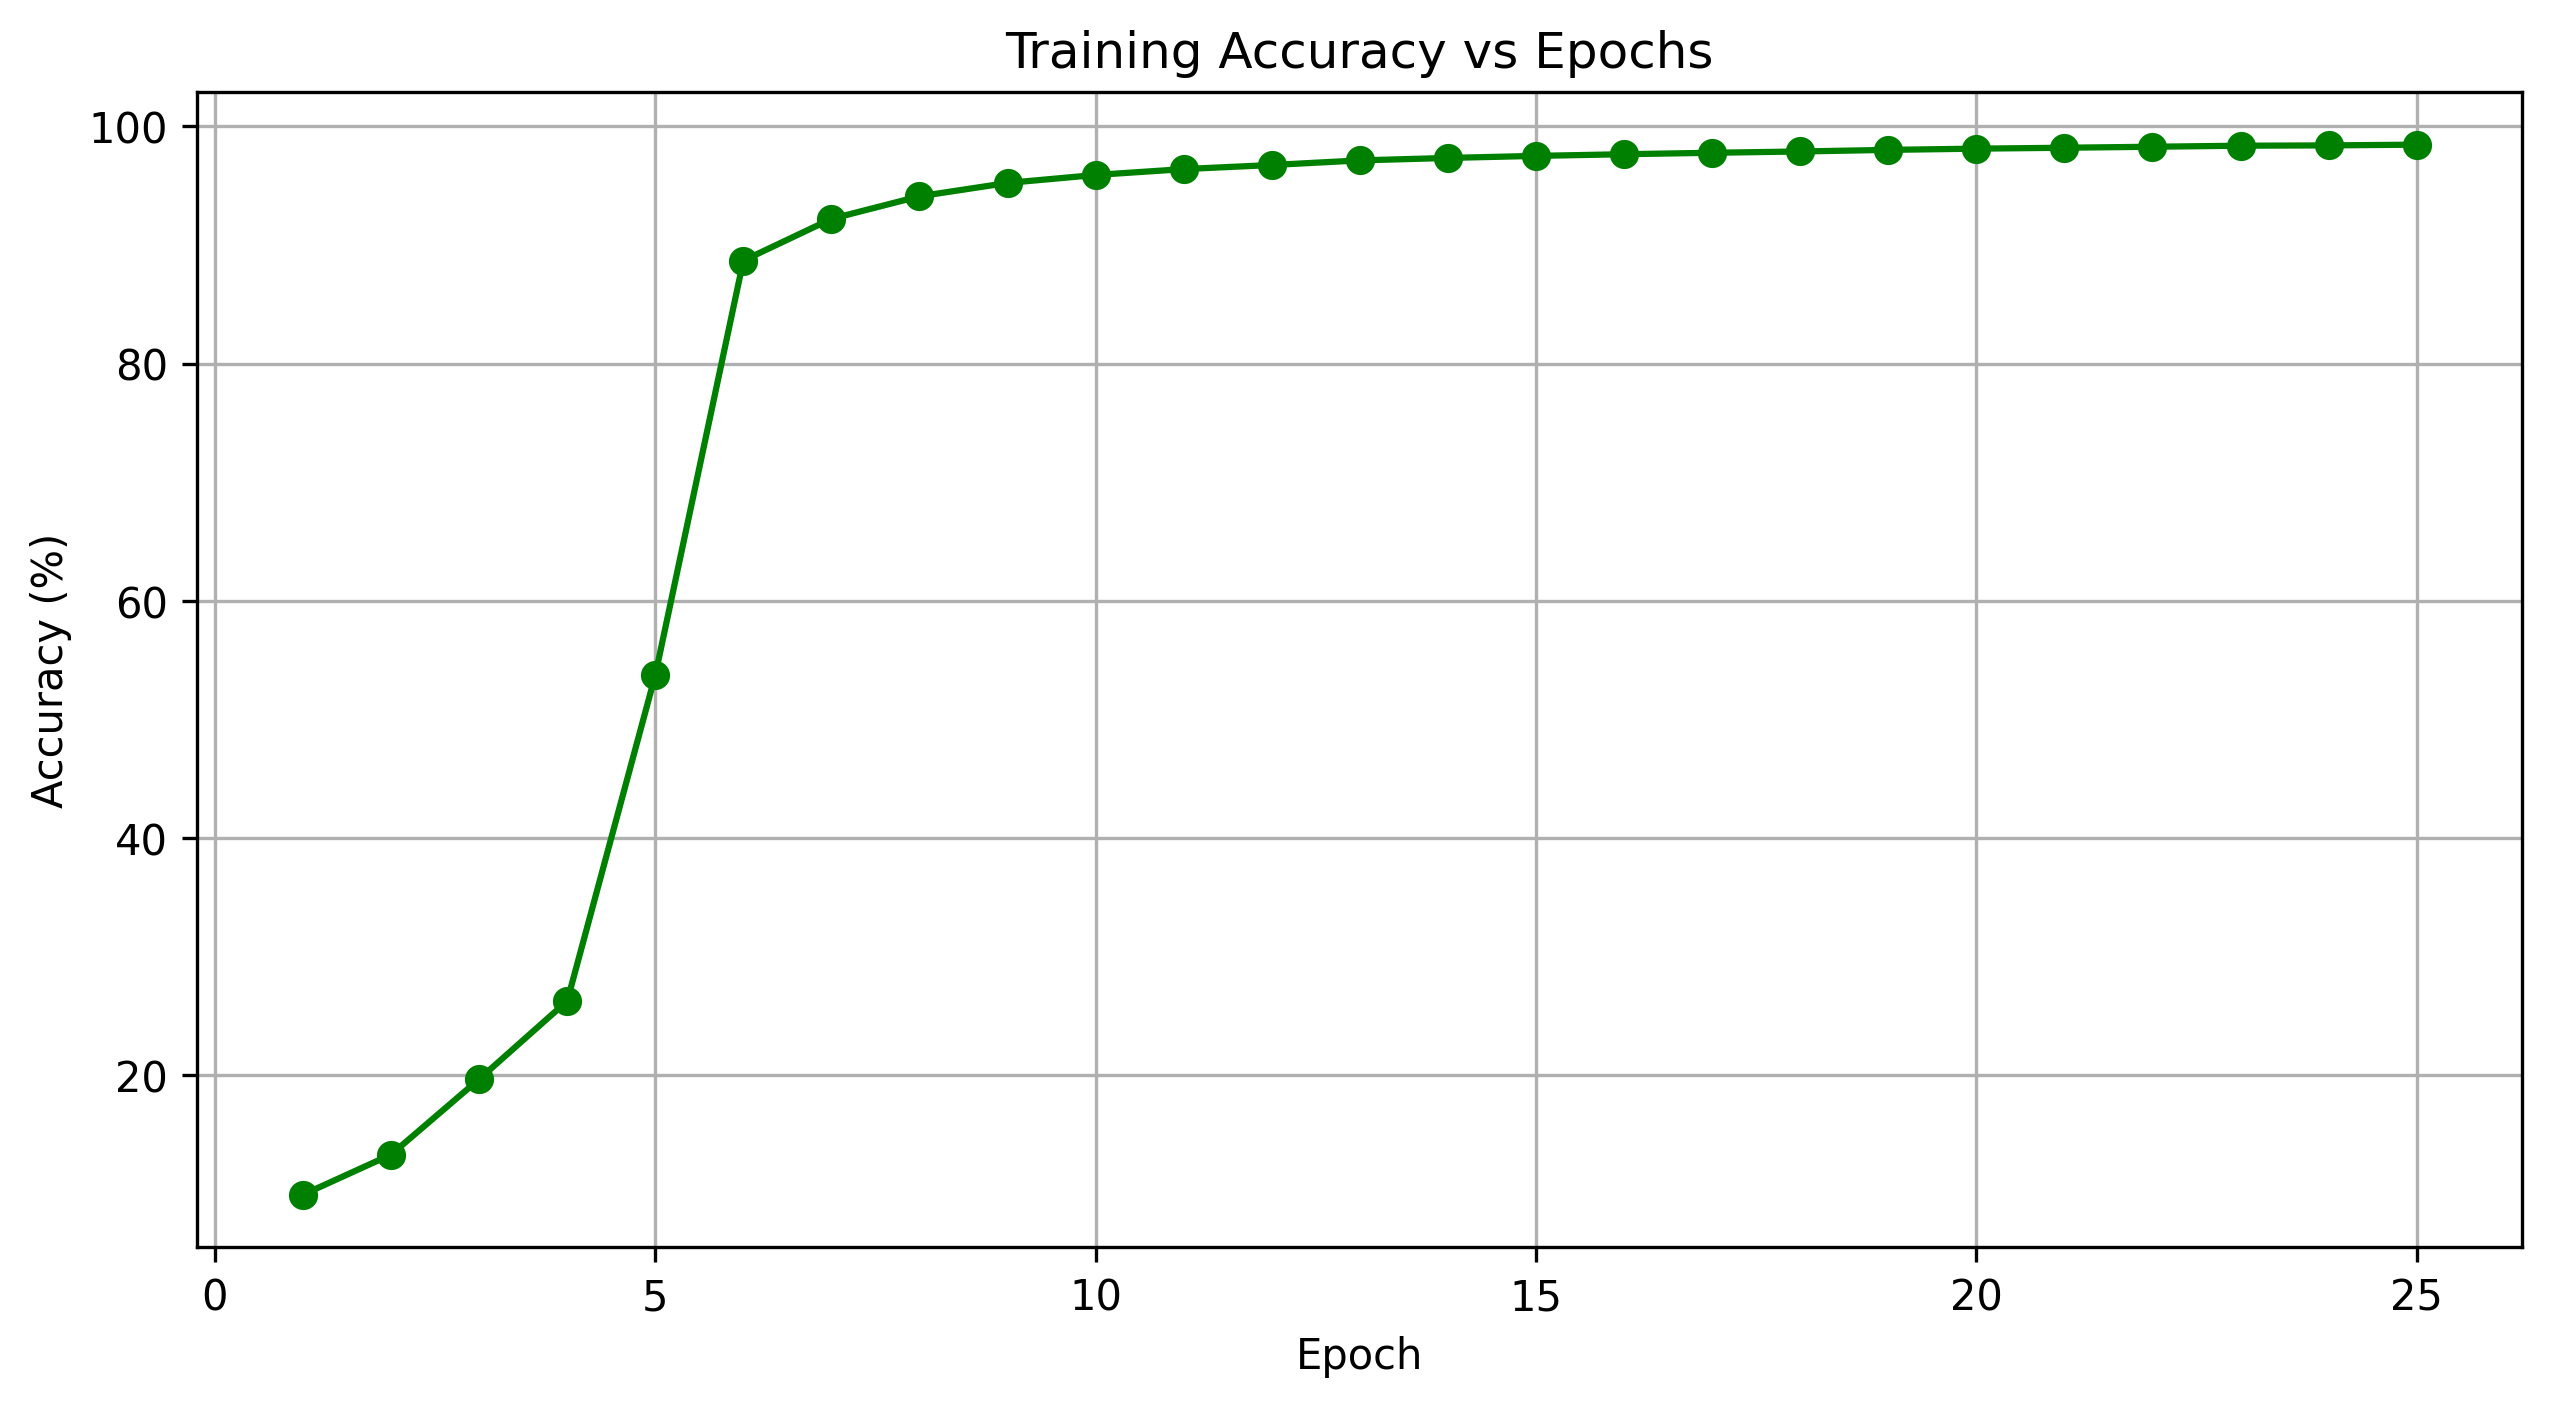
\includegraphics[width=0.9\linewidth]{dense_accuracy_vs_epochs.png}
    \caption{Accuracy vs Epochs for Dense CNN}
    \label{fig:dense-acc}
\end{figure}

\begin{figure}[H]
    \centering
    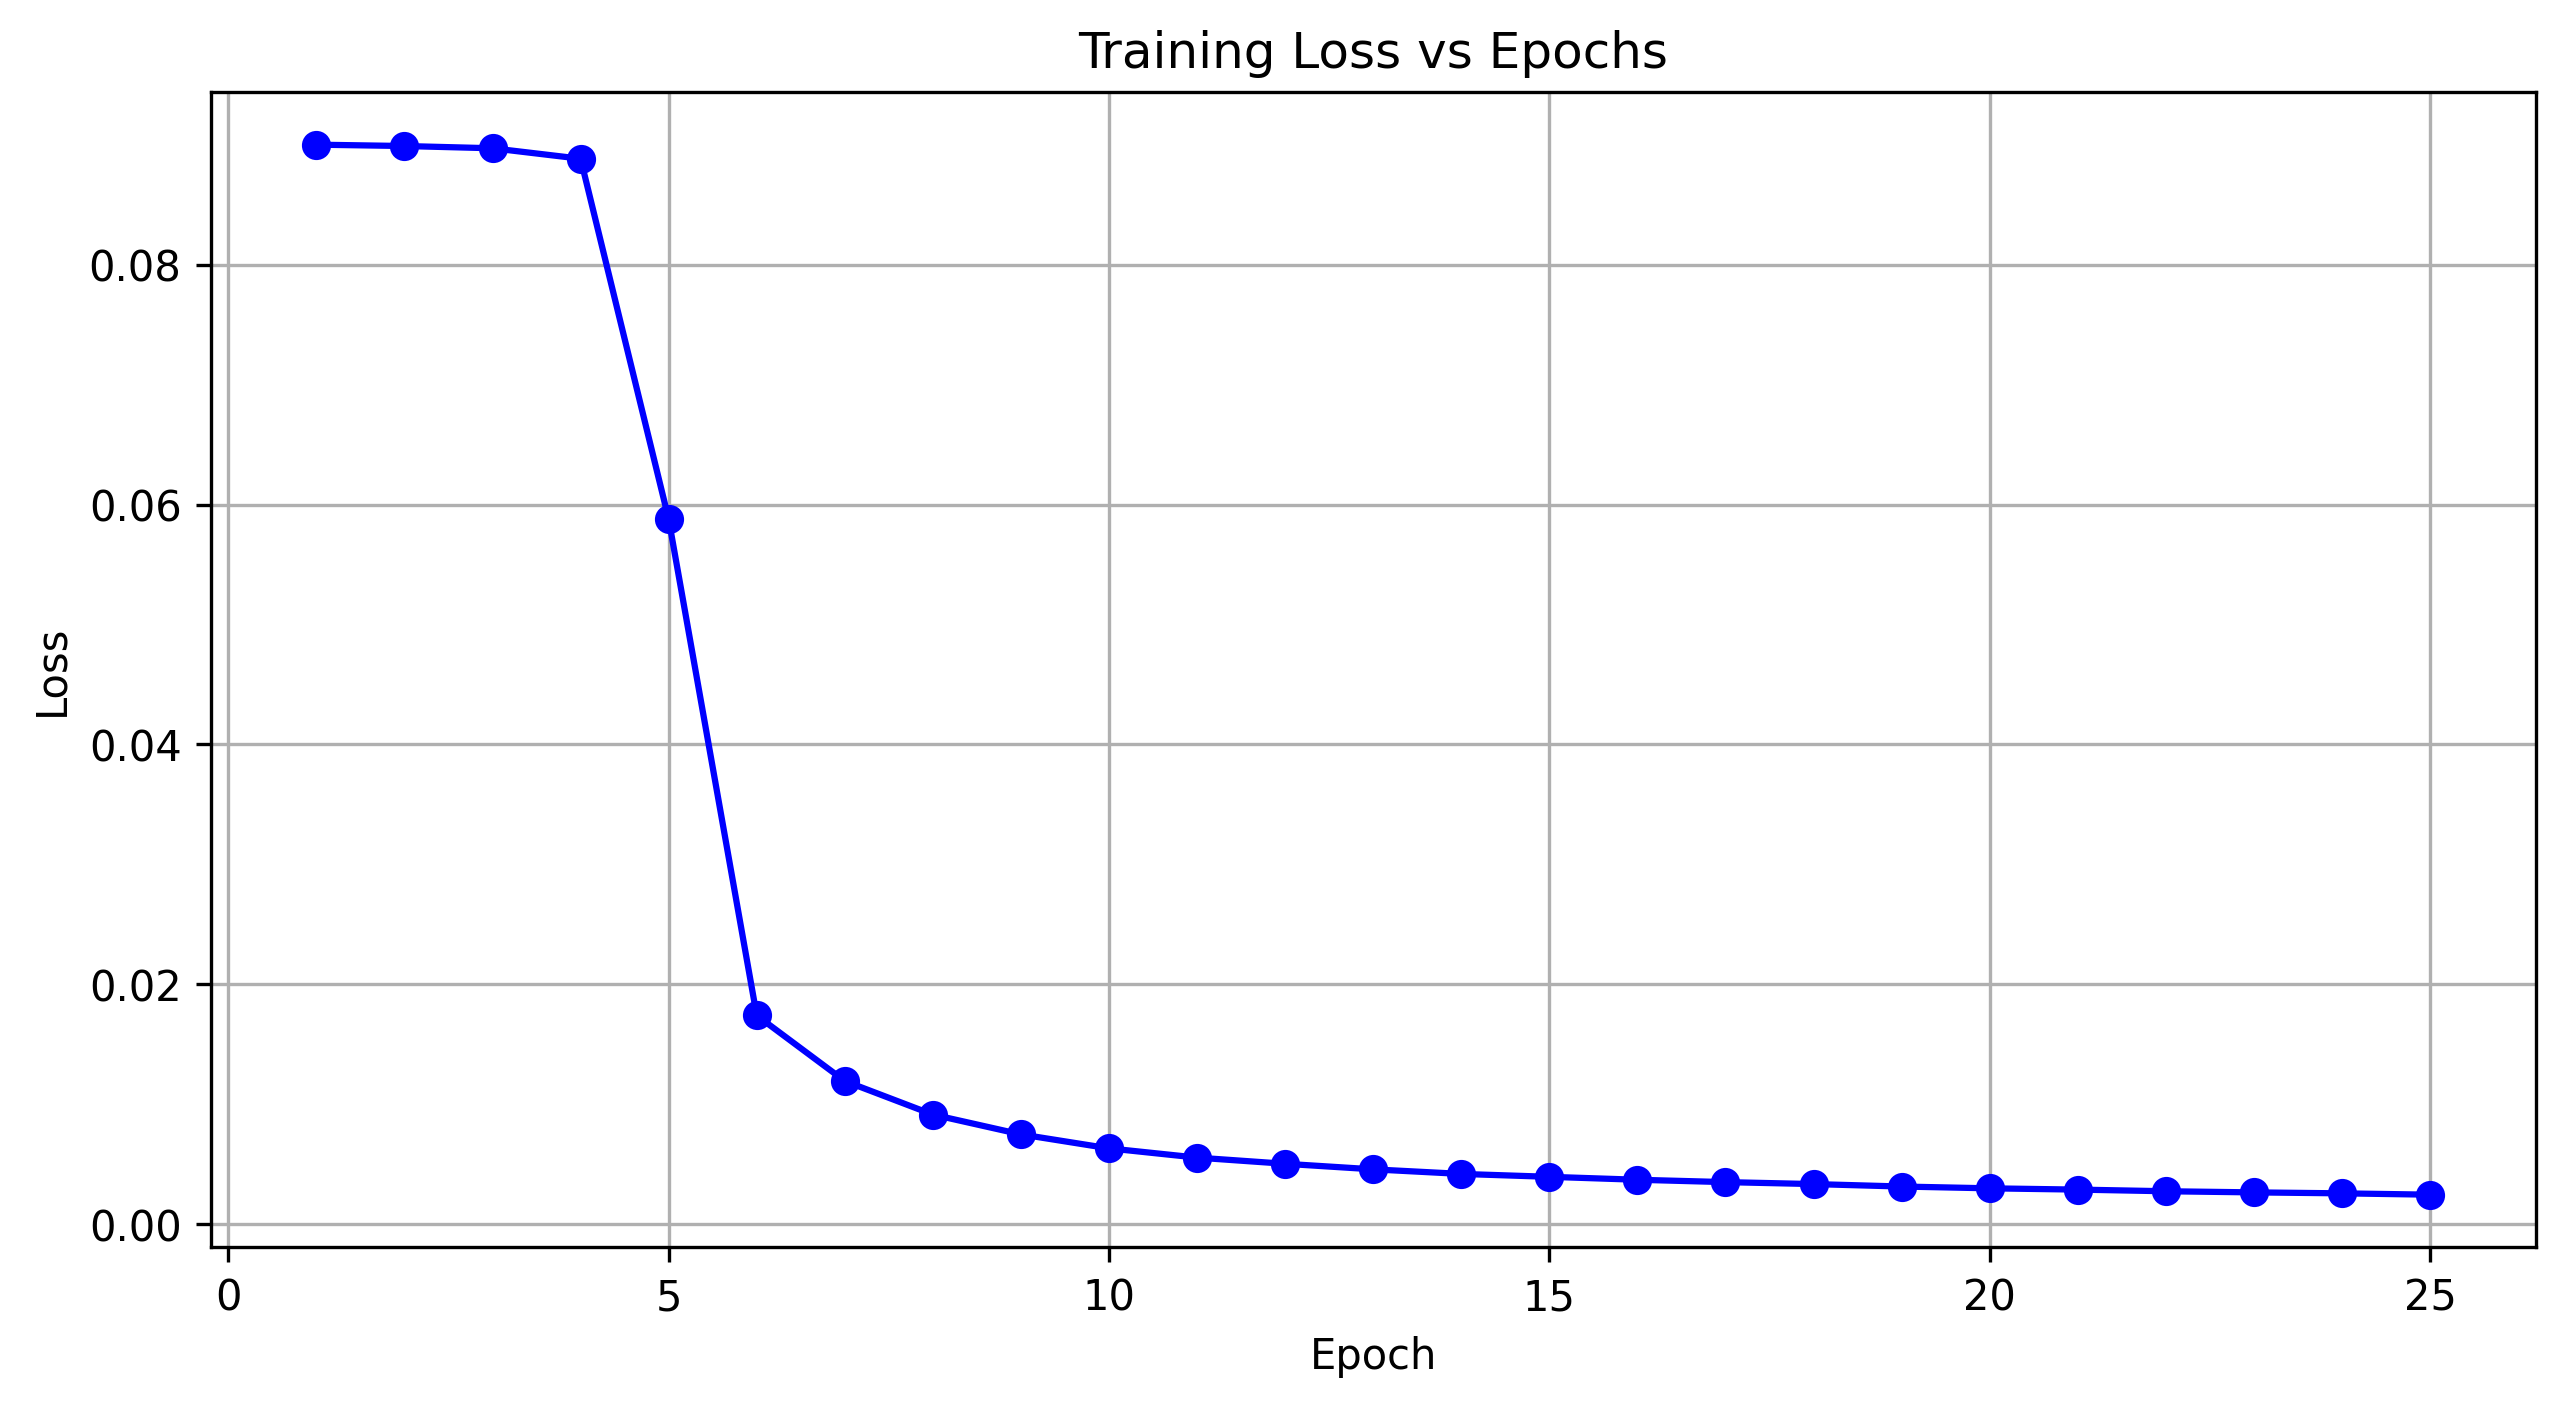
\includegraphics[width=0.9\linewidth]{dense_loss_vs_epochs.png}
    \caption{Loss vs Epochs for Dense CNN}
    \label{fig:dense-loss}
\end{figure}

\newpage

\subsection{LeNet with Depth-Wise Convolution}
Number of Epochs: 70\\
Optimizer: SGD with lr=0.01, momentum=0.9\\
Batch Size: 50\\

\begin{figure}[H]
    \centering
    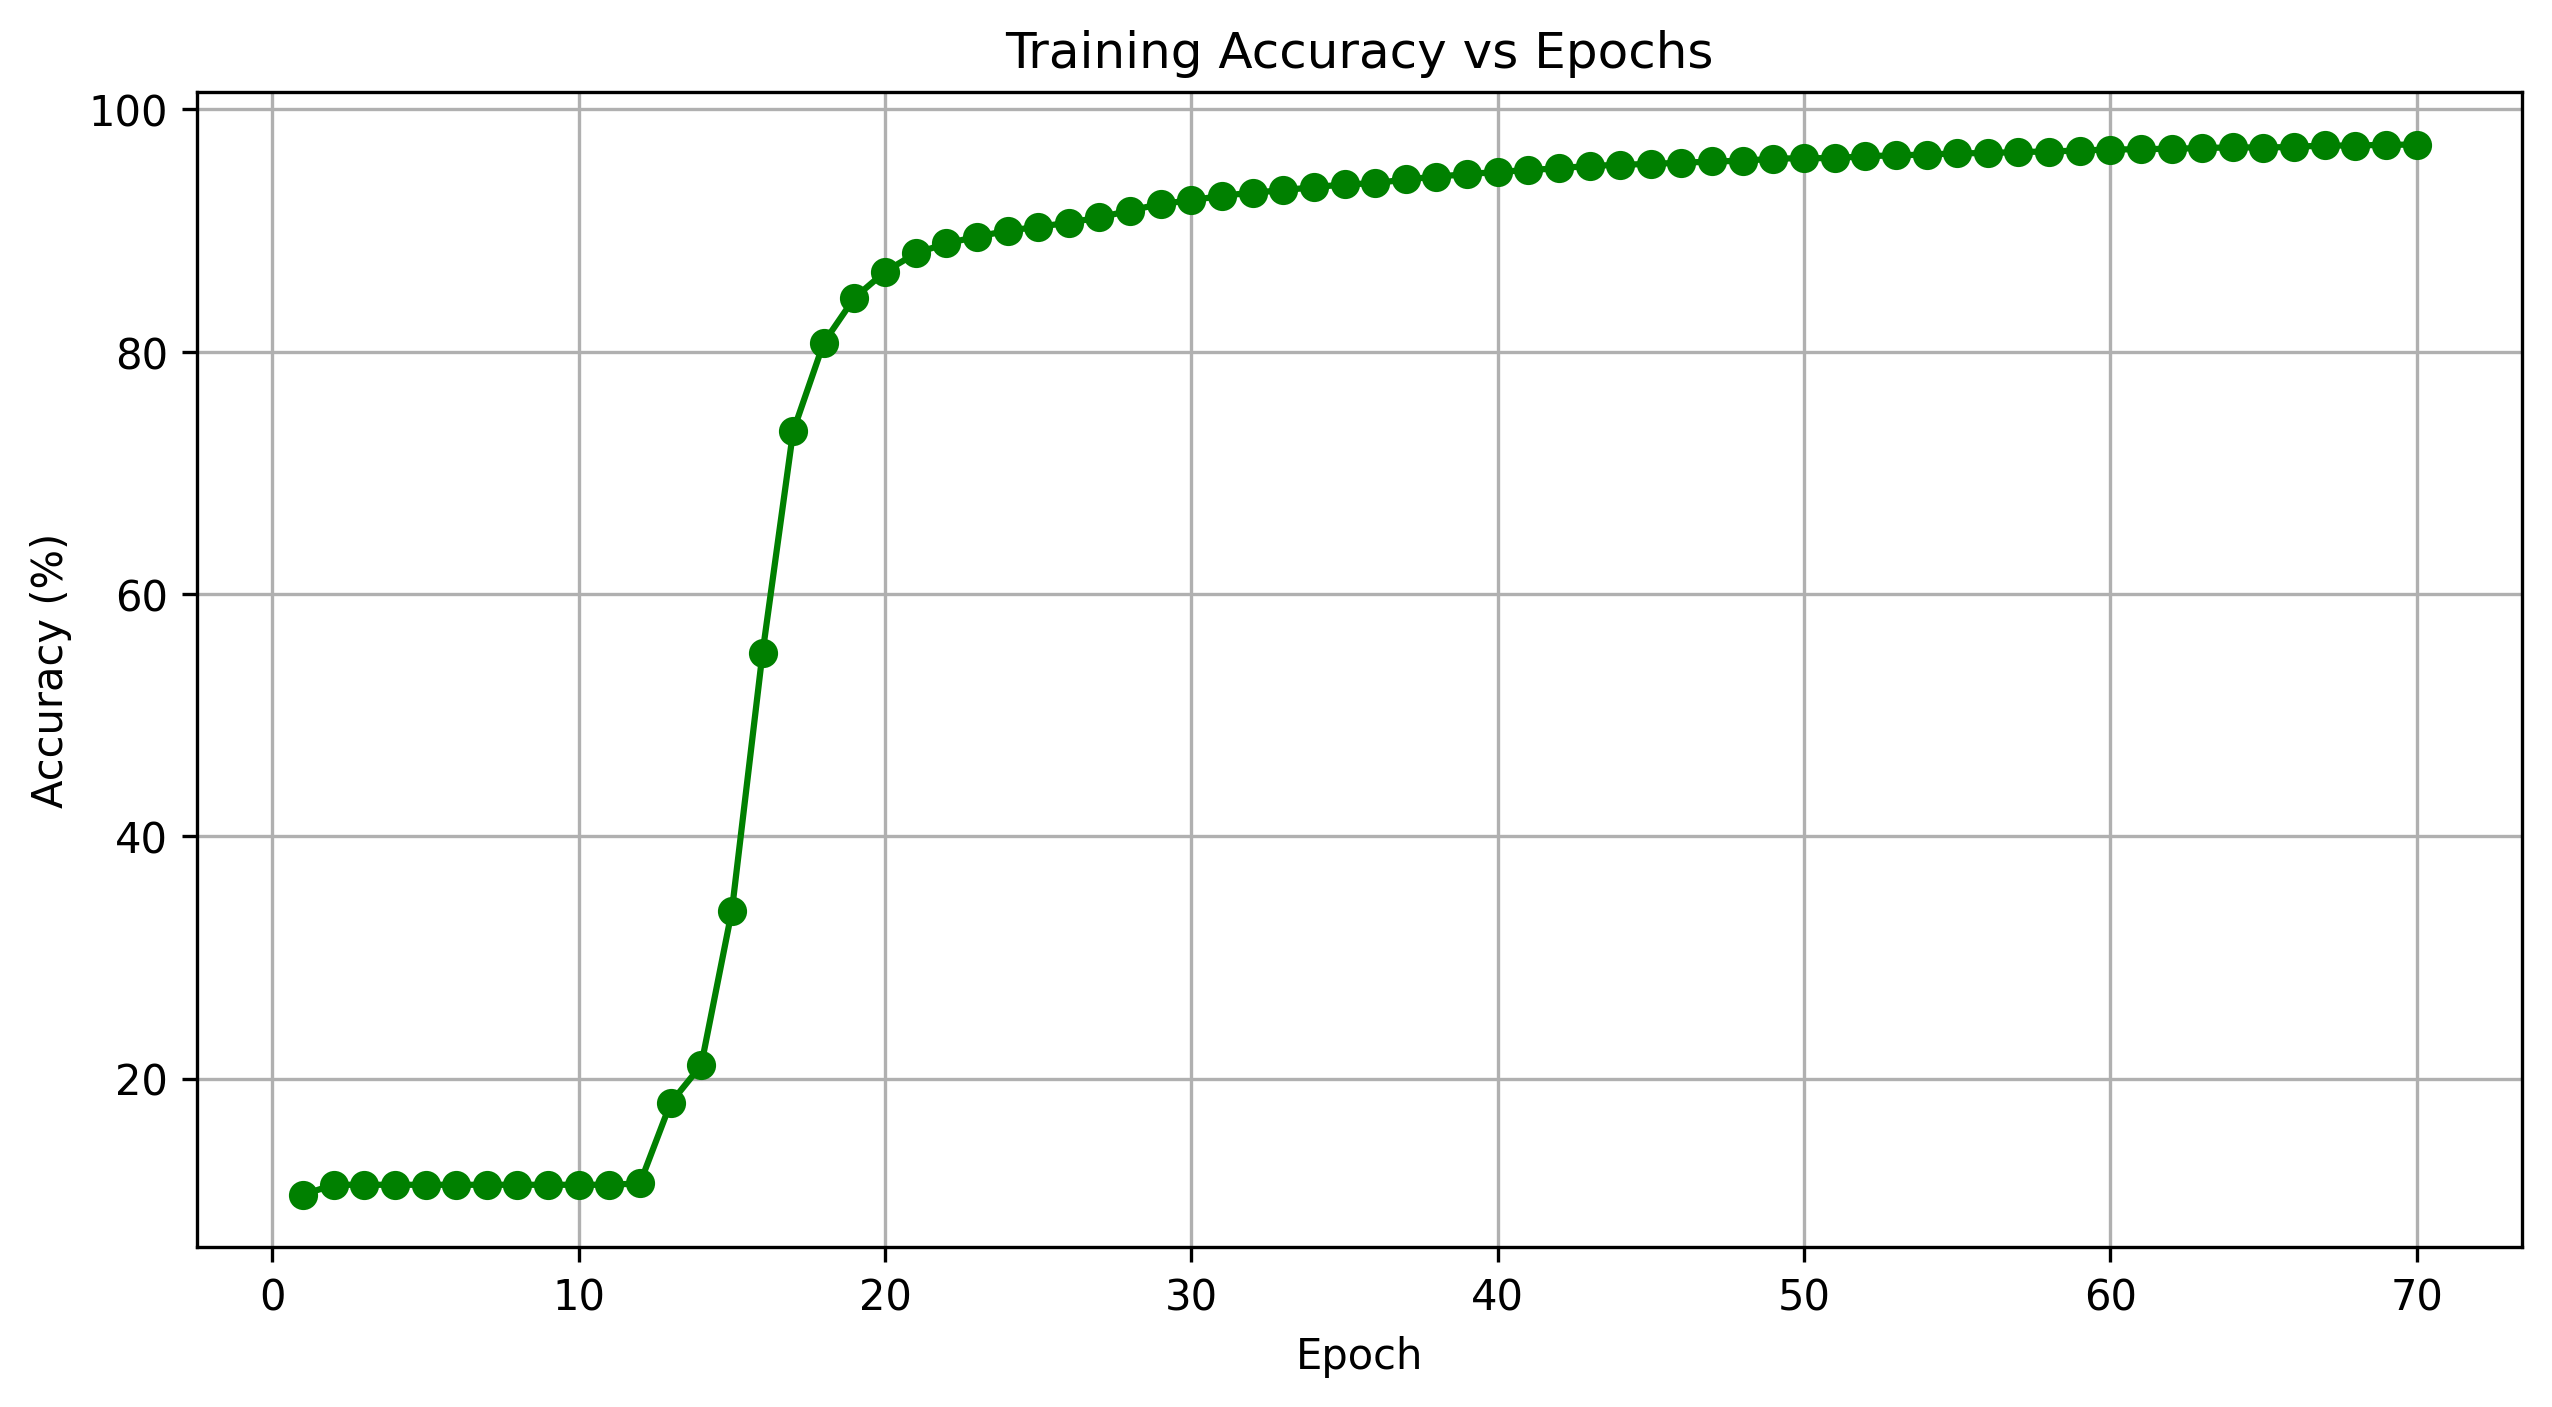
\includegraphics[width=0.9\linewidth]{depthwise_accuracy_vs_epochs.png}
    \caption{Accuracy vs Epochs for Depth-Wise Separable CNN}
    \label{fig:depthwise-acc}
\end{figure}


\begin{figure}[H]
    \centering
    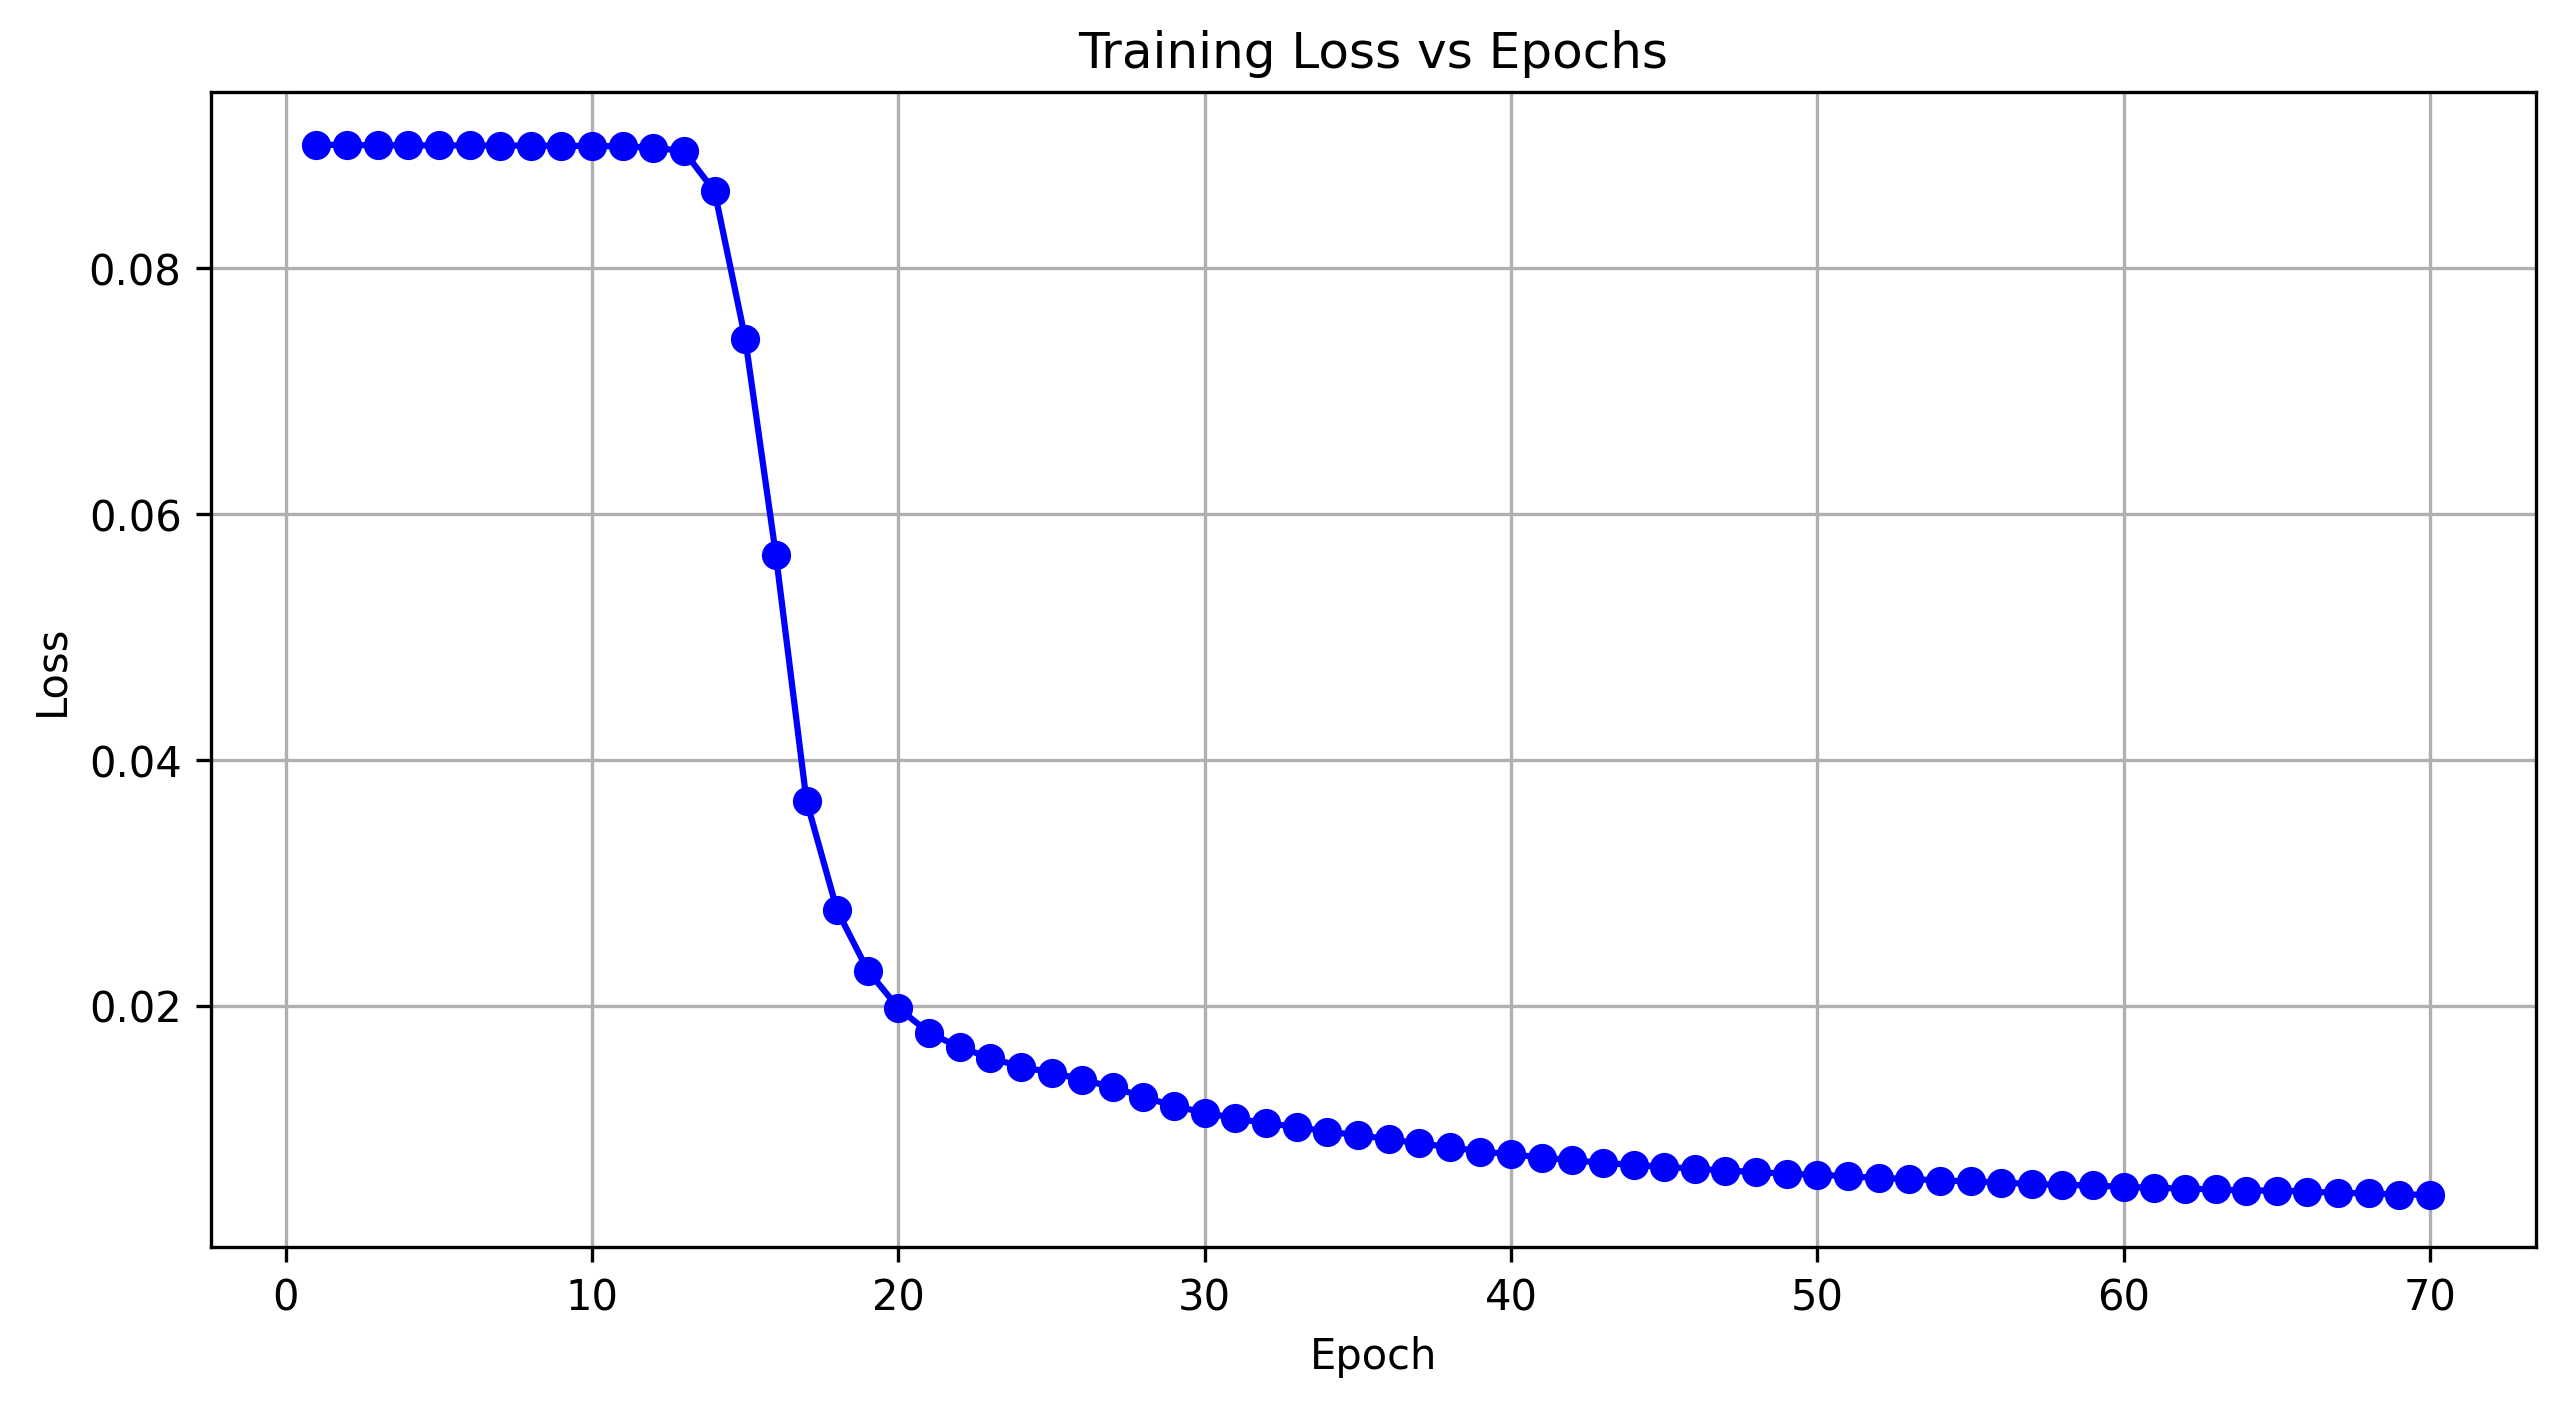
\includegraphics[width=0.9\linewidth]{depthwise_loss_vs_epochs.png}
    \caption{Loss vs Epochs for Depth-Wise Separable CNN}
    \label{fig:depthwise-loss}
\end{figure}

\subsection{Number of MACs}

We will consider the following formula to calculate MACs in convolution layers:
\begin{equation}
    \text{MACs} = K \times C_{in} \times H_{k} \times W_{k} \times H_{out} \times W_{out}
\end{equation}
\noindent where $K$ is the Number of Kernels, $C_{in}$ is Input Channels, $H_k/W_k$ are Kernel dimensions, and $H_{out}/W_{out}$ are Output Map dimensions.\\
\\
Pooling layers do not require MAC operations, so we will not consider them in our calculations. Since fully connected layers can be considered as convolution layers with kernel size equal to the input feature map size, we can use the same formula to calculate MACs in fully connected layers as well.

\subsubsection{Dense CNN}

There are two convolution layers and 3 fully connected layers in the Dense CNN architecture. The number of MACs in each layer is as follows:

\begin{itemize}
    \item \textbf{Conv Layer 1:} Input Fmap = $1 \times 32 \times 32$, Output Fmap = $6 \times 28 \times 28$, Kernel Size = $5 \times 5$, Number of Kernels = $6$
    \begin{equation}
        \text{MACs} = 6 \times 1 \times 5 \times 5 \times 28 \times 28 = 117,600
    \end{equation}
    
    \item \textbf{Conv Layer 2:} Input Fmap = $6 \times 14 \times 14$, Output Fmap = $16 \times 10 \times 10$, Kernel Size = $5 \times 5$, Number of Kernels = $16$
    \begin{equation}
        \text{MACs} = 16 \times 6 \times 5 \times 5 \times 10 \times 10 = 240,000
    \end{equation}
    
    \item \textbf{Fully Connected Layer 1:} Input Fmap = $16 \times 5 \times 5$, Output Fmap = $120 \times 1 \times 1$, Kernel Size = $16 \times 5 \times 5$, Number of Kernels = $120$
    \begin{equation}
        \text{MACs} = 120 \times 16 \times 5 \times 5 \times 1 \times 1 = 480,000
    \end{equation}
    
    \item \textbf{Fully Connected Layer 2:} Input Fmap = $120 \times 1 \times 1$, Output Fmap = $84 \times 1 \times 1$, Kernel Size = $120 \times 1 \times 1$, Number of Kernels = $84$
    \begin{equation}
        \text{MACs} = 84 \times 120 \times 1 \times 1 \times 1 \times 1 = 10,080
    \end{equation}
    
    \item \textbf{Fully Connected Layer 3:} Input Fmap = $84 \times 1 \times 1$, Output Fmap = $10 \times 1 \times 1$, Kernel Size = $84 \times 1 \times 1$, Number of Kernels = $10$
    \begin{equation}
        \text{MACs} = 10 \times 84 \times 1 \times 1 \times 1 \times 1 = 840
    \end{equation}
\end{itemize}

Total MACs in Dense CNN = $117,600 + 240,000 + 480,000 + 10,080 + 840 =$ \textbf{848,520}

\subsubsection{Depth-Wise Separable CNN}


There are 3 convolution layers (each with Depth Wise + Point Wise Convolution) and 2 fully connected layers in the Depth-Wise Separable CNN architecture. The number of MACs in each layer is as follows:

\begin{itemize}
    \item \textbf{Depth Wise Conv Layer 1:} Input Fmap = $1 \times 32 \times 32$, Output Fmap = $1 \times 28 \times 28$, Kernel Size = $5 \times 5$, Number of Kernels = $1$
    \begin{equation}
        \text{MACs} = 1 \times 1 \times 5 \times 5 \times 28 \times 28 = 7,000
    \end{equation}
    
    \item \textbf{Point Wise Conv Layer 1:} Input Fmap = $1 \times 28 \times 28$, Output Fmap = $6 \times 28 \times 28$, Kernel Size = $1 \times 1$, Number of Kernels = $6$
    \begin{equation}
        \text{MACs} = 6 \times 1 \times 1 \times 1 \times 28 \times 28 = 4,704
    \end{equation}
    
    \item \textbf{Depth Wise Conv Layer 2:} Input Fmap = $6 \times 14 \times 14$, Output Fmap = $6 \times 10 \times 10$, Kernel Size = $5 \times 5$, Number of Kernels = $6$
    \begin{equation}
        \text{MACs} = 6 \times 6 \times 5 \times 5 \times 10 \times 10 = 90,000
    \end{equation}
    
    \item \textbf{Point Wise Conv Layer 2:} Input Fmap = $6 \times 10 \times 10$, Output Fmap = $16 \times 10 \times 10$, Kernel Size = $1 \times 1$, Number of Kernels = $16$
    \begin{equation}
        \text{MACs} = 16 \times 6 \times 1 \times 1 \times 10 \times 10 = 9,600
    \end{equation}
    
    \item \textbf{Depth Wise Conv Layer 3:} Input Fmap = $16 \times 5 \times 5$, Output Fmap = $16 \times 1 \times 1$, Kernel Size = $5 \times 5$, Number of Kernels = $16$
    \begin{equation}
        \text{MACs} = 16 \times 16 \times 5 \times 5 \times 1 \times 1 = 6,400
    \end{equation}
    
    \item \textbf{Point Wise Conv Layer 3:} Input Fmap = $16 \times 1 \times 1$, Output Fmap = $120 \times 1 \times 1$, Kernel Size = $1 \times 1$, Number of Kernels = $120$
    \begin{equation}
        \text{MACs} = 120 \times 16 \times 1 \times 1 \times 1 \times 1 = 1,920
    \end{equation}
    
    \item \textbf{Fully Connected Layer 1:} Input Fmap = $120 \times 1 \times 1$, Output Fmap = $84 \times 1 \times 1$, Kernel Size = $120 \times 1 \times 1$, Number of Kernels = $84$
    \begin{equation}
        \text{MACs} = 84 \times 120 \times 1 \times 1 \times 1 \times 1 = 10,080
    \end{equation}
    
    \item \textbf{Fully Connected Layer 2:} Input Fmap = $84 \times 1 \times 1$, Output Fmap = $10 \times 1 \times 1$, Kernel Size = $84 \times 1 \times 1$, Number of Kernels = $10$
    \begin{equation}
        \text{MACs} = 10 \times 84 \times 1 \times 1 \times 1 \times 1 = 840
    \end{equation}
\end{itemize}

Total MACs in Depth-Wise Separable CNN = $7,000 + 4,704 + 90,000 + 9,600 + 6,400 + 1,920 + 10,080 + 840 =$ \textbf{129,544}

\subsection{Mathematical Function}

To derive a mathematical function that relates the number of MAC operations for regular and depth wise separable convolutions, we can consider the following:

\begin{itemize}
    \item Let the input feature map have dimensions: $H_{in} \times W_{in} \times C_{in}$
    \item Let the output feature map have dimensions: $H_{out} \times W_{out} \times C_{out}$
    \item Let the kernel size be: $H_k \times W_k \times C_k$
    \item Let the number of kernels be: $N_k$
    \item $N_k = C_{out}$ for a convolution operation since each kernel produces one output channel.
    \item $C_k = C_{in}$ for a convolution operation since each kernel operates on all input channels.
\end{itemize}

For regular convolution, the number of MACs can be calculated as:
\begin{equation}
    \text{MACs}_{\text{regular}} = N_k \times C_k \times H_k \times W_k \times H_{out} \times W_{out}
\end{equation}

This can also be written as:
\begin{equation}
    \text{MACs}_{\text{regular}} = C_{out} \times C_{in} \times H_k \times W_k \times H_{out} \times W_{out}
    \label{eq:macs-regular}
\end{equation}

For Depth-Wise Separable Convolution, we perform two operations: Depth Wise Convolution and Point Wise Convolution:

\begin{itemize}
    \item \textbf{Depth Wise Convolution:} Each input channel is convolved with a single kernel to produce an output channel. We only change the size of the input feature map to match with the desired output feature map, but cross-channel relation is not captured. Thus, $C_{out}$ = $N_k$ = $C_{in}$, $C_k$ = 1. The number of MACs can be calculated as:
    \begin{equation}
        \text{MACs}_{\text{depthwise}} = C_{in} \times 1 \times H_k \times W_k \times H_{out} \times W_{out}
    \end{equation} 
    \item \textbf{Point Wise Convolution:} We take $C_{out}$ number of $1 \times $1 kernels with each kernel having $C_{in}$ channels to capture the cross-channel relation from the output of depth wise convolution. Thus, $N_k$ = $C_{out}$, $C_k$ = $C_{in}$, $W_k$ = 1, $H_k$ = 1. The number of MACs can be calculated as:
    \begin{equation}
        \text{MACs}_{\text{pointwise}} = C_{out} \times C_{in} \times 1 \times 1 \times H_{out} \times W_{out}
    \end{equation}
\end{itemize}

Total MACs for Depth-Wise Separable Convolution can be calculated as:
\begin{equation}
    \text{MACs}_{\text{depthwise separable}} = \text{MACs}_{\text{depthwise}} + \text{MACs}_{\text{pointwise}}
\end{equation}
\begin{equation}
    \text{MACs}_{\text{depthwise separable}} = C_{in} \times H_k \times W_k \times H_{out} \times W_{out} + C_{out} \times C_{in} \times H_{out} \times W_{out}
\end{equation}
Taking $C_{in} \times H_{out} \times W_{out}$ common, we get:
\begin{equation}
    \text{MACs}_{\text{depthwise separable}} = C_{in} \times H_{out} \times W_{out} \times (H_k \times W_k + C_{out})
    \label{eq:macs-depthwise}
\end{equation}

Dividing ~\ref{eq:macs-depthwise} by ~\ref{eq:macs-regular}, we get:
\begin{equation}
    \frac{\text{MACs}_{\text{depthwise separable}}}{\text{MACs}_{\text{regular}}} = \frac{H_k \times W_k + C_{out}}{C_{out} \times H_k \times W_k}
\end{equation}
Shifting terms, we get the final mathematical function that outputs the number of MACs in Depth-Wise Separable Convolution given the number of MACs in Regular Convolution and other parameters:
\begin{equation}
    \text{MACs}_{\text{depthwise separable}} = \text{MACs}_{\text{regular}} \times \left(\frac{1}{W_k \times H_k} + \frac{1}{C_{out}}\right)
\end{equation}

\section{Problem 3}
Given the following parameters:
\begin{itemize}
    \item Input Feature Map: 9 x 6 x 7
    \item Weight Dimensions = 1 x 9 x 3 x 3
    \item Input Buffer Size = 9 elements
    \item Output Buffer Size = 1 element
    \item Weight Buffer Size = 9 elements
\end{itemize}

Therefore, the output feature map dimensions are: 1 x 4 x 5

\subsection{Read/Writes for Weight Stationary Data Flow}

Since we have a weight buffer and input buffer of size 9 elements, we can store one complete kernel channel (3 x 3) and the corresponding 3 x 3 input patch in the buffers.
Each weight buffer will be used to calculate the partial sums for all the output elements using the corresponding input elements. Thus, the inputs will be read multiple times, but the weights will be read only once.
As we move onto the next kernel channel, we will again read all the corresponding input elements and the partial sum values previously calculated. 
Thus, we need to read 3 x 3 weight values 9 times. Inputs are read in 3 x 3 patches 9 times which will happen $W_{out} \times H_{out} = 20$ times since we have 20 output elements.
The partial sum for the output element will be read and written for each MC operation between the weights and the inputs. 
Thus, for the entire convolution, we have:

\begin{itemize}
    \item Weight Reads = $3 \times 3 \times 9 = 81$
    \item Input Reads = $3 \times 3 \times 9 \times 4 \times 5 = 1620$
    \item For output reads/writes, we have two cases:
        \begin{itemize}
            \item For the first pass (Weight Channel 1), the reads are 0, since we don't have any previous partial sums. 
            We calculate the partial sums using the 9 weight and 9 input elements in the buffer and write the output to main memory for each of the 20 output elements.
            \item For passes 2 to 9, we read previous partial sums from memory and write them back. This is done for each of the 20 elements.
            \item Thus, Output Reads = $0 + 20 \times 8 = 160$ and Output Writes = $20 \times 9 = 180$
        \end{itemize}
\end{itemize}

\begin{table}[h]
\centering
    \begin{tabular}{|l|r|r|}
    \hline
    \textbf{Component} & \textbf{Reads} & \textbf{Writes} \\ \hline
    Weights            & 81             & 0               \\ \hline
    Inputs             & 1,620          & 0               \\ \hline
    Outputs            & 160            & 180             \\ \hline
    \textbf{Total}     & \textbf{1,861} & \textbf{180}    \\ \hline
    \end{tabular}
\end{table}

\subsection{Read/Writes for Input Stationary Data Flow}

For the input stationary data flow, we store one element from each of the 9 input channels in the input buffer and one element from each weight channnel in the weight buffer.
For a particular input buffer, we calculate all the partial sums associated with those inputs by reading the weight elements once for every output element.
Every MAC operation for all channels will require the output to be read and written once to the main memory. Thus, for the entire convolution we have:

\begin{itemize}
    \item Weight Reads = $3 \times 3 \times 9 \times 4 \times 5 \times = 1620$
    \item Input Reads = $6 \times 7 \times 9 = 378$
    \item Output Reads = $9 \times 4 \times 5 \times = 180$ since we read the output element once for a MAC operation between 9 inputs and 9 weights.
    Technically, the first pass doesn't read any partial sum, so we read the partial sums for 8 passes, effectively giving $160$ reads.
    \item Output Writes = $9 \times 4 \times 5 \times = 180$ since we write for each MAC operation between 9 inputs and 9 weights.
\end{itemize}

\begin{table}[h]
\centering
    \begin{tabular}{|l|r|r|}
    \hline
    \textbf{Component} & \textbf{Reads} & \textbf{Writes} \\ \hline
    Weights            & 1,620          & 0               \\ \hline
    Inputs             & 378          & 0               \\ \hline
    Outputs            & 180            & 180              \\ \hline
    \textbf{Total}     & \textbf{2178} & \textbf{180}     \\ \hline
    \end{tabular}
\end{table}

\subsection{Output Stationary Data Flow}

Number of Filters = 9 \\
Output Buffer Size = 9 \\
Number of Output Channels = 9 \\

For the output stationary data flow, we store a 3 x 3 patch of input elements in the input buffer and a complete 3 x 3 channel of weights in the weight buffer. 
In the output buffer, we store a single element from each of the 9 channels. We perform a MAC operation between the input and weight buffers to get the partial sum for one output element.
While the input channel is fixed, we cycle through each kernel, reading one channel at a time and store the partial sums for each output element from each channel.
We read the input and weights, channel by channel, to get all the partial sums for each output element.
Thus, we need to read both the input and weight buffers 9 times for each of the 20 output elements.
For the entire convolution, we have:

\begin{itemize}
    \item Weight Reads = $3 \times 3 \times 9 \times \times 9 \times 20 = 14580$
    \item Input Reads = $3 \times 3 \times 9 \times 20 = 1620$. The input buffer is kept fixed until all the MACs with all kernels are complete to get the output for one output element.
    \item Output Reads = $0$ since we don't have any previous partial sums to read, and we store all consecutive partial sums for all 9 output elements in the output buffer until we calculate the final sum for each output element.
    \item We write the output to main memory for each of the 20 output elements in each channel after calculating the final sum using all the weights and input channels.\\
    Thus, Output Writes = $20 \times 9 = 180$
\end{itemize}

\begin{table}[h]
\centering
    \begin{tabular}{|l|r|r|}
    \hline
    \textbf{Component} & \textbf{Reads} & \textbf{Writes} \\ \hline
    Weights            & 14,580          & 0               \\ \hline
    Inputs             & 1620         & 0               \\ \hline  
    Outputs            & 0              & 180            \\ \hline
    \textbf{Total}     & \textbf{16,200} & \textbf{180}     \\ \hline
    \end{tabular}
\end{table}

\subsection{Comparison of Different Data Flows}

The effectiveness of a data flow is a function of its buffer size and the number of elements associated. In the above question, since the weight buffer size was big enough to either store an entire channel or store an element from each channel, the number of reads and writes was minimum for a weight stationary flow. However, as soon as we had multiple kernels and implemented output stationary data flow, the number of weight reads exploded.\\
\\
In general, we have a large number of weights in a convolution operation. Weights are required multiple times for calculating the output elements, since we have to iterate through each input channel and perform MAC. In my opinion, weight-stationary data flow will result in the lowest reads for most of the cases of CNNs.\\
\\
In cases where we have a lot of input elements as compared to the buffer size, then implementing input-stationary can also be a good strategy. However, the output stationary data flow will not provide good optimizations in most of the CNN cases, as the output feature map is always smaller than the input feature map, and the number of output channels is equal to the number of kernels, and for a large number of kernels, implementing weight-stationary would be better.

\section{Problem 4}

Given Parameters for the MLP:\\
\\
Input Layer = 10 Neurons\\
First Hidden Layer = 8 Neurons\\
Number of Weights from Input to First Layer = $10 \times 8 = 80$\\
\\
Second Hidden Layer = 6 Neurons\\
Number of Weights from first hidden layer to second hidden layer = $8 \times 6 = 48$\\
\\
Output Layer = 5 Neurons\\
Number of Weights from second hidden layer to output layer = $6 \times 5 = 30$\\
\\
During a forward pass, when we transition from a layer with $N_1$ neurons to a layer with $N_2$ neurons, each neuron in the second layer undergoes the following:

\begin{itemize}
    \item $N_1$ number of multiplications between the activation value and the associated weight of each neuron in the previous layer.
    \item Summation between all the products. Assuming that an addition operation consists of 2 numbers, we need to perform $N_1 - 1$ operations.
    \item A single non-linear operation on the summed activation.
\end{itemize}\\
\\
Given data for each operation:

\begin{itemize}
    \item Multiplication: 8 Cycles
    \item Addition: 2 Cycles
    \item Non-Linear: 1 Cycle
\end{itemize}
\\
With this context, we can analyze the different hardware implementations and calculate the corresponding number of cycles.

\subsection{Naive Hardware}

This is a full neuron implementation on the chip, where multiple neurons can be processed parallely. If we assume full capability, then the hardware is big enough to process all the neurons in a single layer simultaneously. This will be a pipelined execution, where the subsequent layers will have to wait for the outputs from the previous layer. Thus, we can say that the number of cycles for an entire layer is equal to the number of cycles required by a single neuron. \\

The bottleneck here is that each neuron has a single multiplier which can perform only one dot-product at a time, requiring 8 cycles. However, as we perform the subsequent multiplications, the additions can happen in parallel, so that only the last addition adds to the latency. Thus, for a layer with $N$ inputs, the neuron has to sequentially perform $N$ multiplications (8 cycles each), 1 addition (2 cycles), and 1 non-linear operation (1 cycle).

This can be calculated as:
\begin{equation}
    N_{cycles} = N_{inputs} * 8 \text{ (Multiplication)} + 2 \text{ (Last Addition)} + 1 \text{ (Non-Linear)} 
\end{equation}
Or, to simplify,
\begin{equation}
    N_{cycles} = 8 \times N_{inputs} + 3
\end{equation}

Now, for each layer transition, we can calculate total cycles:

\begin{table}[H]
    \centering
    \begin{tabular}{|l|c|c|}
        \hline
        \textbf{Layer} & \textbf{$N_{inputs}$} & \textbf{Total Cycles} \\
        \hline
        First Hidden & 10 & 83 \\
        \hline
        Second Hidden & 8 & 67 \\
        \hline
        Output & 6 & 51 \\
        \hline
    \end{tabular}
    \label{tab:naive-cycles}
\end{table}

\begin{equation}
    \text{Total Cycles} = 83 + 67 + 51 = \textbf{201}
\end{equation}

\subsection{Hardware with NFUs}

With the implementation of NFUs, we get the capability to process multiple inputs in parallel. Assuming a full-capability system, we can process all the inputs in a layer simultaneously. This will again be a pipelined execution, where the inputs will be multiplied parallely in NFU1, all the products will be sent to NFU2 where they will be added in one-shot, and then passed to NFU3 for the non-linear operation.\\

The bottleneck here is that each output neuron has to be processed sequentially since there is a single set of NFUs. However, we can achieve parallelism by processing the subsequent output neuron as soon as the previous one is finished with its multiplication operation in NFU1. This ensures that all additions and non-linear cycles overlap with the multiplication cycles, except for the last neuron. Thus, for a layer with $N$ output neurons, the hardware needs to perform  $N$ multiplications (8 cycles), 1 addition (2 cycles), and 1 non-linear operation (1 cycle).\\

This can be written as:
\begin{equation}
    N_{cycles} = N_{outputs} \times 8 + 3
\end{equation}

\begin{table}[H]
    \centering
    \begin{tabular}{|l|c|c|}
        \hline
        \textbf{Layer} & \textbf{$N_{outputs}$} & \textbf{Total Cycles} \\
        \hline
        Input & 8 & 67 \\
        \hline
        First Hidden & 6 & 51 \\
        \hline
        Second Hidden & 5 & 43 \\
        \hline
    \end{tabular}
    \label{tab:naive-cycles}
\end{table}

\begin{equation}
    \text{Total Cycles} = 67 + 51 + 43 = \textbf{161}
\end{equation}

\end{document}